%
% File acl2019.tex
%
%% Based on the style files for ACL 2018, NAACL 2018/19, which were
%% Based on the style files for ACL-2015, with some improvements
%%  taken from the NAACL-2016 style
%% Based on the style files for ACL-2014, which were, in turn,
%% based on ACL-2013, ACL-2012, ACL-2011, ACL-2010, ACL-IJCNLP-2009,
%% EACL-2009, IJCNLP-2008...
%% Based on the style files for EACL 2006 by 
%%e.agirre@ehu.es or Sergi.Balari@uab.es
%% and that of ACL 08 by Joakim Nivre and Noah Smith

\documentclass[11pt,a4paper]{article}
\usepackage{graphicx}
\usepackage{subcaption}
\graphicspath{ {imgs/} }
\usepackage[table,xcdraw]{xcolor}
\usepackage[hyperref]{acl2019}
\usepackage{times}
\usepackage{latexsym}
\usepackage{multirow}
\usepackage{url}

\aclfinalcopy % Uncomment this line for the final submission
%\def\aclpaperid{***} %  Enter the acl Paper ID here

%\setlength\titlebox{5cm}
% You can expand the titlebox if you need extra space
% to show all the authors. Please do not make the titlebox
% smaller than 5cm (the original size); we will check this
% in the camera-ready version and ask you to change it back.

\newcommand\BibTeX{B\textsc{ib}\TeX}

\title{Reddit Classification}

\author{Uberti-Bona Mar\'{i}n, L. G. \\
  Department of Data Science \\
  and Knowledge Engineering \\
  Maastricht University \\\And
  Marrades Furquet, J. R. \\
  Department of Data Science \\
  and Knowledge Engineering \\
  Maastricht University}

\date{}

\begin{document}
\maketitle

% Introduction
\section{Introduction}
\label{sec:introduction}
Since we spend most of our lectures browsing through Reddit, we have decided to make
something productive out of it: a multi-use bot that helps us browse, comment and post
on our favorite subreddits in order to make us earn as much karma as possible and
improve our experience on this social media.

% Literature Review
\section{Literature Review}
\label{sec:literature_review}
Where is our FASOS slave?

% Tasks
\section{Tasks}
\label{sec:tasks}
Every community within Reddit is called a subreddit. We decided to focus in the
following subreddits:
\begin{enumerate}
	\item \textit{r/AmItheAsshole}. In this subreddit users ask other users if, given a
	specific situation they made a mistake or not. The task would be to determine for a
	given post if the user did make a mistake or not.
	\item Tips subreddits: \textit{r/LifeProTips}, \textit{r/ShittyLifeProTips},
	\textit{r/UnethicalLifeProTips}, \textit{r/IllegalLifeProTips}\footnote{Hereinafter, to be
	called \textit{lpt}, \textit{slpt}, \textit{ulpt} and \textit{ilpt}, respectively.}. With these
	subreddits we would like to build a \textit{tip classifier}. That is, a model which
	determines on which subreddit a specific tip should be. 
\end{enumerate}

% Reddit API
\section{Reddit API}
\label{sec:reddit_api}
In order to avoid retrieval constraints, it was decided to use \texttt{pushshift.io} and its
API. Nevertheless, a Reddit developer account was created in order to obtain keys for
authorization purposes.\\

The decision of using the API instead of finding an already existing dataset is 
due to the fact that some of these files are unbalanced, outdated or contain unnecessary information. Thus, making customizaed requests ensures the collection of balanced and updated data. 

% Am I the Asshole?
\section{Am I the Asshole?}
\label{sec:aita}

% ProTips
\section{ProTips}
\label{sec:protips}
% Data retrieved
Using the Reddit API, $100$k posts were retrieved. Out of those, $90$k were distributed
evenly among \textit{lpt}, \textit{slpt} and \textit{ulpt}. 

% Validation of models
\begin{figure*}[h!] % The asterisk means "hey span all the page, so avoid multicols"
\centering
	% Naive Bayes (BOW) validation
	\begin{subfigure}[h!]{0.3\textwidth}
		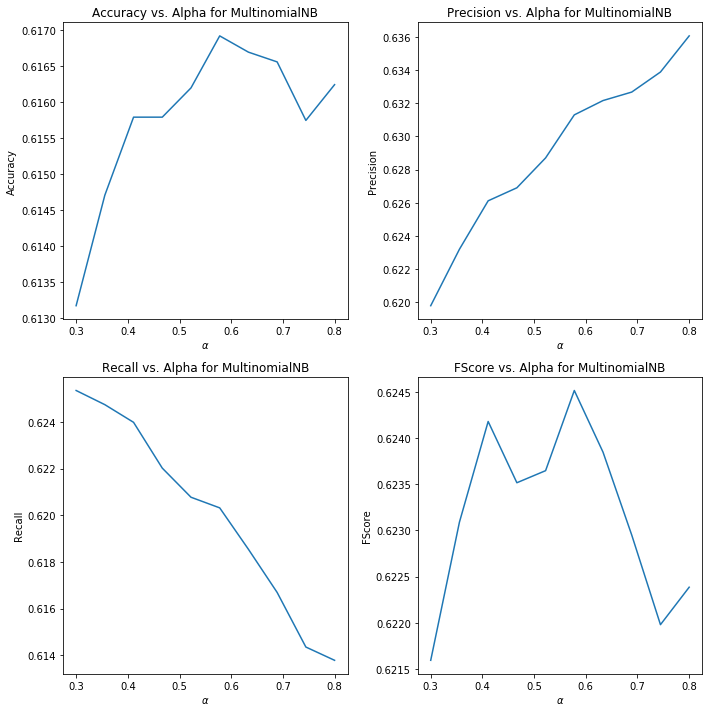
\includegraphics[width=\linewidth]{plots_nb.png}
		\caption{Naive Bayes (BOW)}
		\label{fig:nb_val}
	\end{subfigure}
	~
	% SVM (Word2Vec) validation
	\begin{subfigure}[h!]{0.3\textwidth}
		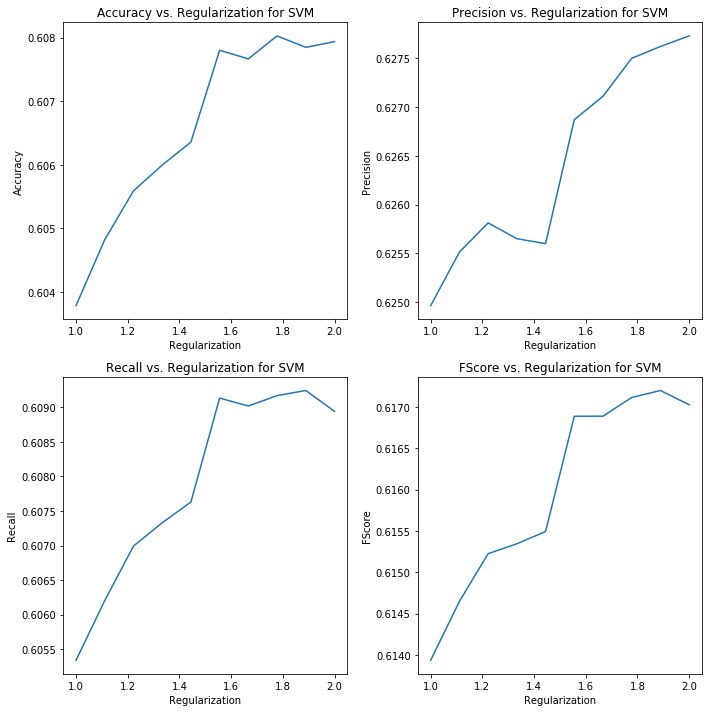
\includegraphics[width=\linewidth]{plots_svm1.png}
		\caption{SVM (Word2Vec)}
		\label{fig:svm1_val}
	\end{subfigure}
	~
	% SVM (Pre-trained Word2Vec) validation
	\begin{subfigure}[h!]{0.3\textwidth}
		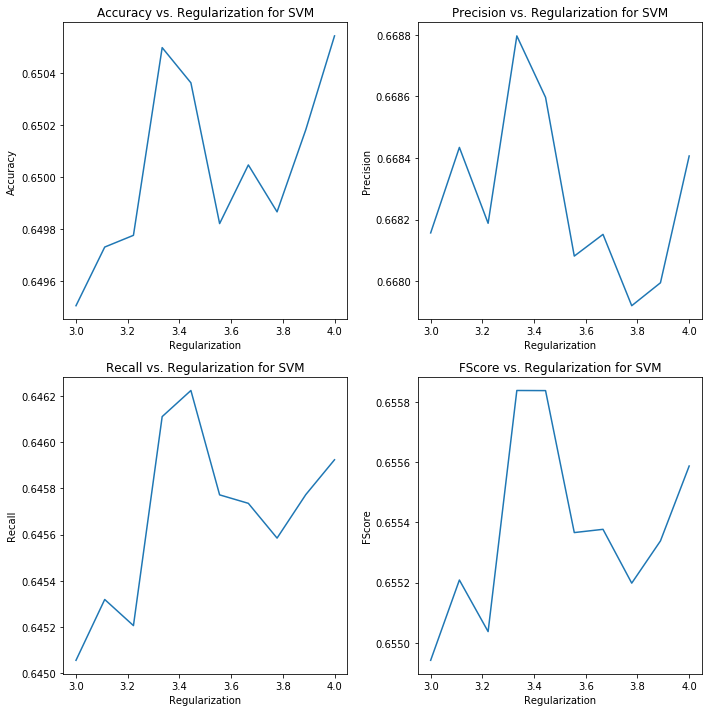
\includegraphics[width=\linewidth]{plots_svm2.png}
		\caption{SVM (Pre-trained Word2Vec)}
		\label{fig:svm2_val}
	\end{subfigure}
	\caption{Validation of models in ProTips}
	\label{fig:models_val}
\end{figure*}

% Naive Bayes (BOW) Confusion Matrix
\begin{table*}[h!]
\centering
\begin{tabular}{c|c|c|c|c|}
\cline{2-5}
                                                            & \cellcolor[HTML]{EFEFEF}\textbf{Pred. ilpt} & \cellcolor[HTML]{EFEFEF}\textbf{Pred. lpt} & \cellcolor[HTML]{EFEFEF}\textbf{Pred. slpt} & \cellcolor[HTML]{EFEFEF}\textbf{Pred. ulpt} \\ \hline
\multicolumn{1}{|c|}{\cellcolor[HTML]{EFEFEF}\textbf{ilpt}} & 2280                                        & 124                                        & 213                                         & 704                                         \\ \hline
\multicolumn{1}{|c|}{\cellcolor[HTML]{EFEFEF}\textbf{lpt}}  & 347                                         & 6041                                       & 1871                                        & 1715                                        \\ \hline
\multicolumn{1}{|c|}{\cellcolor[HTML]{EFEFEF}\textbf{slpt}} & 198                                         & 1563                                       & 6059                                        & 2122                                        \\ \hline
\multicolumn{1}{|c|}{\cellcolor[HTML]{EFEFEF}\textbf{ulpt}} & 607                                         & 1085                                       & 1840                                        & 6443                                        \\ \hline
\end{tabular}
\caption{Confusion Matrix for Naive Bayes (BOW) in ProTips.}
\label{table:nb_cf}
\end{table*}

% SVM (Word2Vec) Confusion Matrix
\begin{table*}[h!]
\centering
\begin{tabular}{c|c|c|c|c|}
\cline{2-5}
                                                            & \cellcolor[HTML]{EFEFEF}\textbf{Pred. ilpt} & \cellcolor[HTML]{EFEFEF}\textbf{Pred. lpt} & \cellcolor[HTML]{EFEFEF}\textbf{Pred. slpt} & \cellcolor[HTML]{EFEFEF}\textbf{Pred. ulpt} \\ \hline
\multicolumn{1}{|c|}{\cellcolor[HTML]{EFEFEF}\textbf{ilpt}} & 2072                                        & 259                                        & 322                                         & 663                                         \\ \hline
\multicolumn{1}{|c|}{\cellcolor[HTML]{EFEFEF}\textbf{lpt}}  & 214                                         & 6649                                       & 1730                                        & 1391                                        \\ \hline
\multicolumn{1}{|c|}{\cellcolor[HTML]{EFEFEF}\textbf{slpt}} & 107                                         & 2058                                       & 5700                                        & 2071                                        \\ \hline
\multicolumn{1}{|c|}{\cellcolor[HTML]{EFEFEF}\textbf{ulpt}} & 427                                         & 1621                                       & 1714                                        & 6203                                        \\ \hline
\end{tabular}
\caption{Confusion Matrix for SVM (Word2Vec) in ProTips.}
\label{table:svm1_w2v}
\end{table*}

% SVM (Pre-trained Word2Vec) Confusion Matrix
\begin{table*}[h!]
\centering
\begin{tabular}{c|c|c|c|c|}
\cline{2-5}
                                                            & \cellcolor[HTML]{EFEFEF}\textbf{Pred. ilpt} & \cellcolor[HTML]{EFEFEF}\textbf{Pred. lpt} & \cellcolor[HTML]{EFEFEF}\textbf{Pred. slpt} & \cellcolor[HTML]{EFEFEF}\textbf{Pred. ulpt} \\ \hline
\multicolumn{1}{|c|}{\cellcolor[HTML]{EFEFEF}\textbf{ilpt}} & 2087                                        & 195                                        & 355                                         & 682                                         \\ \hline
\multicolumn{1}{|c|}{\cellcolor[HTML]{EFEFEF}\textbf{lpt}}  & 147                                         & 6966                                       & 1584                                        & 1283                                        \\ \hline
\multicolumn{1}{|c|}{\cellcolor[HTML]{EFEFEF}\textbf{slpt}} & 100                                         & 1766                                       & 6063                                        & 2006                                        \\ \hline
\multicolumn{1}{|c|}{\cellcolor[HTML]{EFEFEF}\textbf{ulpt}} & 394                                         & 1337                                       & 1511                                        & 6729                                        \\ \hline
\end{tabular}
\caption{Confusion Matrix for SVM (Pre-trained Word2Vec) in ProTips.}
\label{table:svm2_w2v}
\end{table*}

% Final Measures
\begin{table*}[h!]
\centering
\begin{tabular}{|c|c|c|c|c|c|c|c|c|}
\hline
\rowcolor[HTML]{DDDDDD} 
\textbf{Repr.}                                                                                  & \textbf{Classifier}           & \textbf{Lapl.}       & \textbf{Reg.} & \textbf{Accuracy}       & \textbf{Avg.} & \textbf{Precision} & \textbf{Recall} & \textbf{FScore} \\ \hline
\cellcolor[HTML]{EFEFEF}                                                                                 &                               &                        &                         &                         & macro              & 0.64               & 0.64            & 0.64            \\ \cline{6-9} 
\multirow{-2}{*}{\cellcolor[HTML]{EFEFEF}BOW}                                                            & \multirow{-2}{*}{Naive Bayes} & \multirow{-2}{*}{0.58} & \multirow{-2}{*}{-}     & \multirow{-2}{*}{62.70\%} & micro              & 0.63               & 0.63            & 0.63            \\ \hline
\cellcolor[HTML]{EFEFEF}                                                                                 &                               &                        &                         &                         & macro              & 0.64               & 0.62            & 0.63            \\ \cline{6-9} 
\multirow{-2}{*}{\cellcolor[HTML]{EFEFEF}Word2Vec}                                                       & \multirow{-2}{*}{SVM}         & \multirow{-2}{*}{-}    & \multirow{-2}{*}{1.78}  & \multirow{-2}{*}{62.12\%} & micro              & 0.62               & 0.62            & 0.62            \\ \hline
\cellcolor[HTML]{EFEFEF}                                                                                 &                               &                        &                         &                         & macro              & 0.68                   & 0.65                & 0.66                \\ \cline{6-9} 
\multirow{-2}{*}{\cellcolor[HTML]{EFEFEF}\begin{tabular}[c]{@{}c@{}}Pre-trained\\ Word2Vec\end{tabular}} & \multirow{-2}{*}{SVM}         & \multirow{-2}{*}{-}    & \multirow{-2}{*}{4.00}  & \multirow{-2}{*}{65.79\%} & micro              & 0.66                   &               0.66  & 0.66                \\ \hline
\end{tabular}
\caption{Performance measures for employed methods in ProTips.}
\label{table:measures}
\end{table*}

% Conclusions
\section{Conclusions}
\label{sec:conclusions}

% Bibliography
\nocite{*}
\bibliography{acl2019}
\bibliographystyle{acl_natbib}

% Appendix
\appendix

%\section{Tables}
%\label{sec:tables}
% PROTIPS

\section{Supplemental Material}
\label{sec:supplemental}
Blah blah blah


\end{document}
